\section{Threats and Challenges}

A seccusefull test has three creterions tp fullfill. First, it has to be \emph{reproducible} in order for others to replecate. Second, the results should be \emph{accurate}, which means each time we rerun the test we are expecting the same results. Finally, it should \emph{represent} the real world. In other words, the conclusions brought from the experemnt should be valide outside the expermentation as well. In our case the real world is the production enviroment, Therefore our experements should reflect what is happening in the production environements.
In this section we will dig deeper in each aspect, present what has been done by others and ourselfs as well, and finally we will propose some perspectives, to make the experements better .


%%%%%%%%% preliminary taughts and section structure 
% The need of reproducibility in our field - software optimization based on empirical studies -

% The importance of Virtualisation for reproducibility \cite{howe_virtual_2012}
% some of the most important parts are
% - fewer constraints on research methods
% - on-demand backups
% - virtual Machines as Publications
% - more Variables captured

\subsection{Reproducibiliy}

One of the most challenges which face the reaserchers is the reproducibility of their tests.Actually many results are not reproducible \footnote{Trouble at the lab, The Economist, 19 October 2013;  www.economist.com/news/briefing/ 21588057-scientists-think-science-self-correcting- alarming-degree-it-not-trouble.}, which let to a \emph{replication crisis}.When this crisis hit most of the empirical studies,most of the reviews now includes reproducibility as one of the minimal standard for judging scientific \cite{peng2011reproducible}. one of the creterions for a reproducidibility is the publication of the dataset and the algorithm run on the raw data to condlude the results. There is even some disagreement about what the terms "reproducibility" or "replicability" by themselves mean \cite{goodman2016does} .According to \cite{echtler2018open} \emph{replicability} extends \emph{reproducibility} to the ability to collect a new raw dataset comparable to the original one by reexecuting the experiment under similar condition, Instead of just the ability to get the same results by ruruning the statistical analyses on the orginal data set.

In this area, reproducibility might be achieved by ensuring the same execution settings of physical nodes, virtual machines, clusters or cloud environments.
However, when it comes to measuring the energy consumption of a system, applying acknowledged guidelines and carefully repeating the same benchmark can nonetheless lead to different energy footprints not only on homogeneous nodes, but even within a single node.


One major problem that hinders the reproducibility of the empirical tests is the interaction with the external environment, either as concurency or dependencies. Therefore testers won't have the same results unless they duplicate the same environment.


\subsection{accuracy}
according to oxford, \emph{accuracy} means \href{https://www.lexico.com/definition/accuracy}{"technical The degree to which the result of a measurement, calculation, or specification conforms to the correct value or a standard"}.
Compare with precision. In our case this means the ability to run the benchmark multiple times with a low variation.

Recently, the research community has been investigating typical "crimes" in systems benchmarking and established guidelines for conducting robust and reproducible evaluations~\cite{DBLP:journals/corr/abs-1801-02381}.

In theory, using identical CPU, same memory configuration, similar storage and networking capabilities, should increase the accuracy of the measures. Unfortunately, this is not possible  when it comes to measuring the energy consumption of a system. applying the benchmarking guidelines and repeating the same experiment with in the same configuration are not enought to reproduce the the same energy measures,not only between identical machines but even within the same machine.
This difference---also called \emph{energy variation} (EV)---has become a serious threat to the accuracy of experimental evaluations.
\begin{figure}%[!htb]
    \center{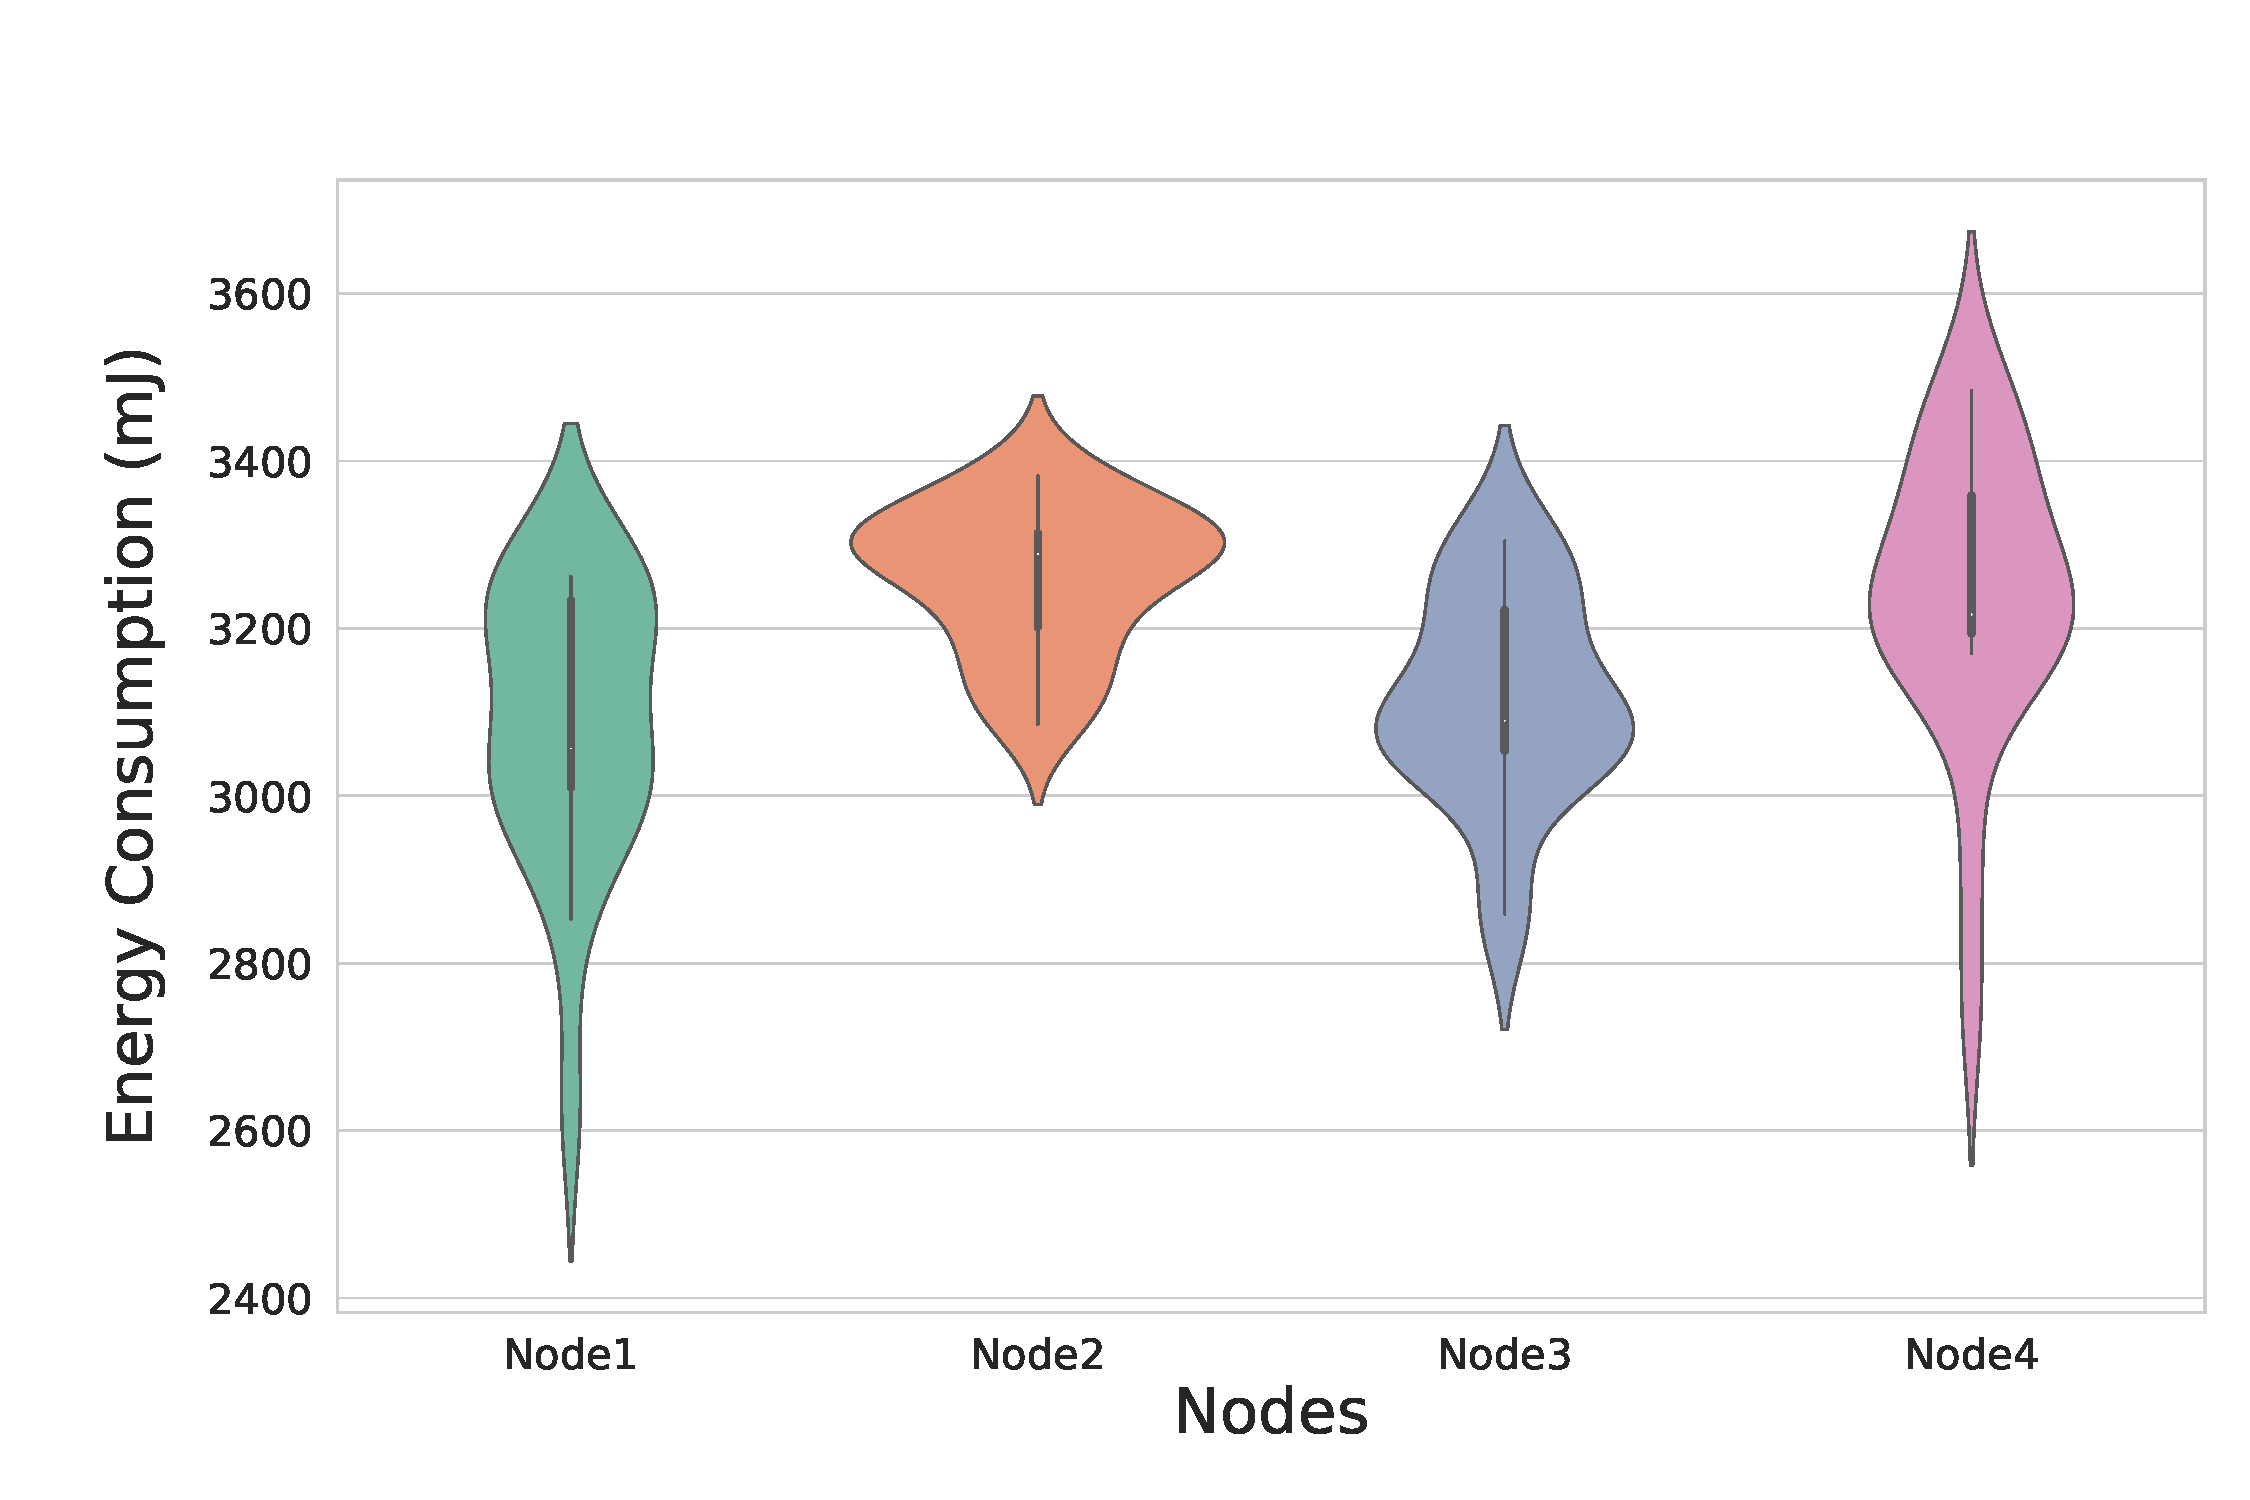
\includegraphics[width=.9\linewidth]{imgs/motivation}}
    \caption{CPU energy variation for the benchmark \textsf{CG}}\label{fig:motivation}
\end{figure}

%TODO:  rephrase this figure, maybe change it a little bit 
Figure~\ref{fig:motivation} illustrates this variation problem as a violin plot of $20$ executions of the benchmark \emph{Conjugate Gradient} (\textsf{CG}) taken from the \emph{NAS Parallel Benchmarks} (NBP) suite~\cite{Bailey:1991:NPB:125826.125925}, on $4$ nodes of an homogeneous cluster (the cluster \textsf{Dahu} described in Table~\ref{table:g5k}) at 50\,\% workload.
we can observe a large variation of the energy consumption, not only among homogeneous machiness, but also at the scale of a single machines, reaching up to $25\,\%$ in this example.

Some reaserchers started investigating the hardware impact of the energy variation of power consumption. As an example we cite ~\cite{borkar_designing_2005,tschanz_adaptive_2002} who reported that the main cause of the variation of the power consumption between different machines is due to the \textbf{CMOS} manufacturing process of transistors in a chip.
\cite{heinrich_predicting}. decribed this variation as a set of parameters such as CPU Frequency and the termal effect.


\subsection{representativeness}
As obvious as it seems, the reason of the doing tests is to validate ideas so we can use them in the real life. Howerver this is means that those tests have to repesent reality somehow.
Basically when we want to test something we create a mock up version of the situation that we want it to wrok. But how can we assure that the test is representative ?. honestly i don't know. and we can't generalize this. but there are some works that have been done for this.
First we can talk about the benchmarking and their selection, then we will talk about the tress test for some applications. and finally we will bring this representativeness in our case and how can we get closer to the energy consumption behaviour of our software between the test environement and the production one.

As Stephen M. Blackburn et al cited in their paper "evaluate collaboratory" \cite{stephen_evaluate_2012} one of major pitfalls of the measurement contexts is the inconsistancy which is translated here with the fact that the production context is not the same as the testing one.

another difficult part for practicioners to generlize their claimes that they have got in the lab outside is the the the workloads. are they appripriate ? are they consistent and are they reproducible ?. To answer those questions the community agreed on some well known benchmarks that they represents an aspect of the the production world. we can site as an exemple the Dacapo set and Renaissance for JAVA applciations. the CLBG benchmark set for programming langauges.
Although they  do not cover all the cases. the community agrees on them. for the moment

In addition to those benchmarks a new category of testings has been born to simulate the worst case of the production enviromenet, Stress tests, are tests meant to evaluate the behaviour of a software under extreme situations.
we can cite as an exemple Gatling for web application and stress-ng for hardwares.
%% YEP I KNOW, THIS IS JUST FOR ME TO READ IT LATER AND GIVE A BETTER CONTEXT



